\begin{frame}
    \titlepage
\end{frame}

\begin{frame}[c]{Apresentação}
    \begin{itemize}
        \item Professor Rodrigo de Farias Gomes
        \item Telefone (somente mensagens): (92) 9 9405-1724
        \item E-mail: shpnft@gmail.com
    \end{itemize}
\end{frame}

\begin{frame}{Ementa}
    \begin{itemize}
        \item Equilíbrio Estático (somente Química Industrial)
        \item Fluidos 
        \item Oscilações 
        \item Ondas em meio material
        \item Ondas sonoras
        \item Temperatura e calor
        \item Primeira lei da termodinâmica
        \item Teoria cinética dos gases
        \item Segunda lei da temodinâmica
        \item Ciclo de Carnot
    \end{itemize}
\end{frame}

\begin{frame}{Avaliação}
    \begin{itemize}
        \item A avaliação será na forma de 3 notas: \(N_1\), \(N_2\) e \(N_3\)
        \item A média dos exercícios escolares (\(MEE\)) será dada por
            \[
                MEE=\frac{N_1+N_2+N_3}{3}
            \]
        \item Se \(MEE \geq 8,0\), então a média final (\(MF\)) será igual à \(MEE\)
        \item Se \(MEE < 8,0\), então
            \[
                MF=\frac{2\times MEE+PF}{3}
            \]
            onde PF é a nota da \textbf{prova final}
        \item Se \(MF \geq 5,0\) e a frequência em sala for maior que 75\%, o aluno está aprovado
    \end{itemize}
\end{frame}

\begin{frame}[c]{Livro texto}
    \begin{center}
        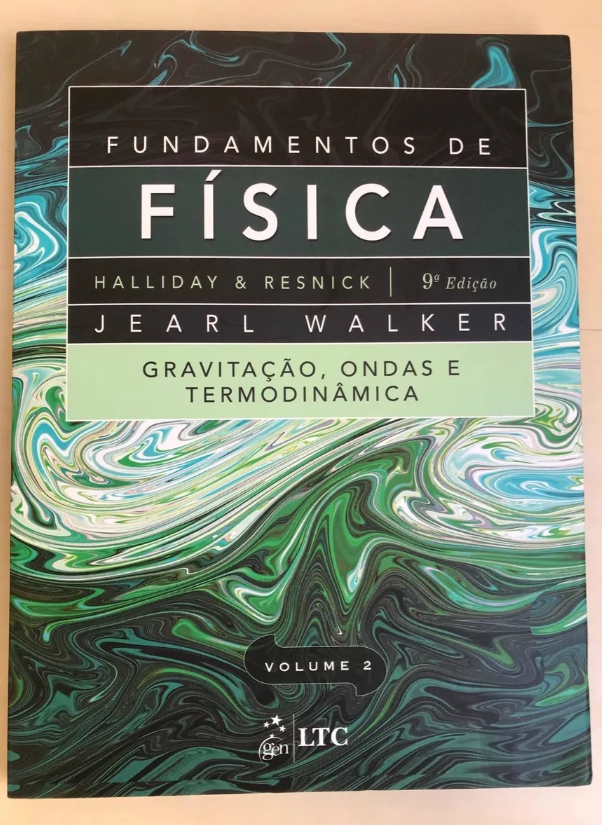
\includegraphics[width=0.33\textwidth]{images/halliday_9.png}
        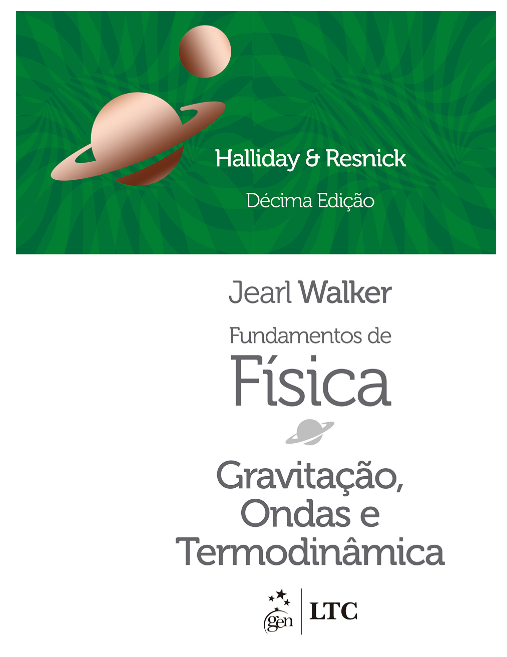
\includegraphics[width=0.33\textwidth]{images/halliday_10.png}
    \end{center}
\end{frame}

\begin{frame}{Força e torque}
    \begin{itemize}
        \item Forças causam variação no movimento \textbf{translacional} 
        \item Torques causam variação no movimento \textbf{rotacional}
    \end{itemize}
    \begin{center}
        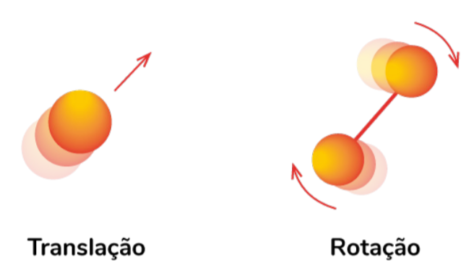
\includegraphics[width=6cm]{images/translação-rotação.png}
    \end{center}
    \pause
    Dessa forma, o que é necessário para que um corpo rígido esteja em \textbf{equilíbrio estático}?
\end{frame}

\begin{frame}{Equilíbrio estático}
    \begin{itemize}[<+->]
        \item A força externa resultante que atua sobre o corpo deve ser nula: 
            \[
                \sum \vec{F}=\vec{0} \implies
                \begin{cases}
                    \sum F_x =0 \\ \sum F_y =0 \\ \textcolor{blue}{\sum F_z =0}
                \end{cases}
            \]

        \item O torque externo resultante deve ser nulo: 
            \[
                \sum \vec{\tau}=\vec{0} \implies
                \begin{cases}
                    \textcolor{blue}{\sum \tau_x =0} \\
                    \textcolor{blue}{\sum \tau_y =0} \\
                    \sum \tau_z =0
                \end{cases}
            \]
    \end{itemize}
\end{frame}

\begin{frame}{Atividade}
    \begin{center}
        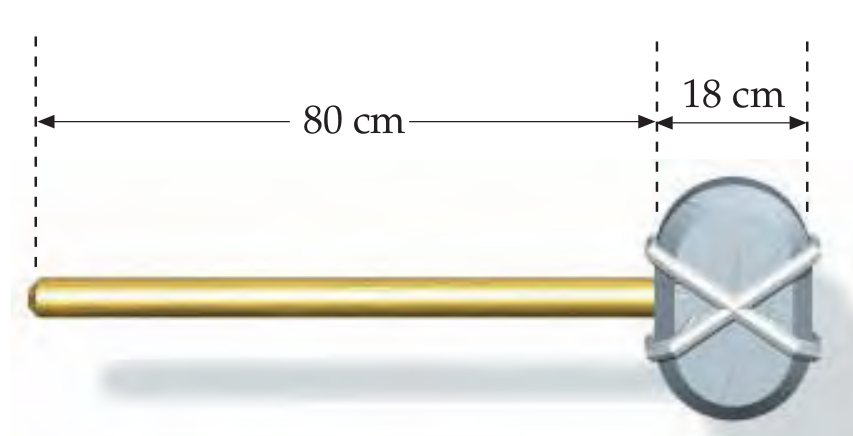
\includegraphics[width=0.5\textwidth]{images/thor}
    \end{center}
    Na figura acima, se a cabeça do martelo pesa \SI{8}{kg} e o cabo pesa \SI{2.5}{kg}, a que distância da extremidade 
    esquerda do martelo devemos amarrar um fio para que ele fique na horizontal quando pendurado? Considere tanto 
    a cabeça quanto o cabo do martelo \textbf{uniformes}

    \pause

    \begin{itemize}
        \item Data de entrega: 20/10
        \item Vale 1 ponto extra na \(N_1\) (nota máxima 10)
    \end{itemize}
\end{frame}
